\documentclass{beamer}
\usetheme{default}

\usepackage{graphicx}
\usepackage{multicol}
\usepackage{fancyvrb}

\newcommand{\bi}{\begin{itemize}}
\newcommand{\ii}{\item}
\newcommand{\ei}{\end{itemize}}

\newcommand{\bframe}[1]{\begin{frame}[fragile]{#1}}




\title{IF notes}
\subtitle{based on {\em The Craft of Adventure, 2nd ed.}, Graham Nelson\\
 and {\em Twisty Little Passages}, Nick Montfort}
\author{Geoffrey Matthews}


\begin{document}
\begin{frame}
\maketitle
\end{frame}
\bframe{Prehistory}
\begin{itemize}
\item Stephen Bishop
\item Explorer, Mammoth Cave, 1820-1857
\end{itemize}

\resizebox{3in}{!}{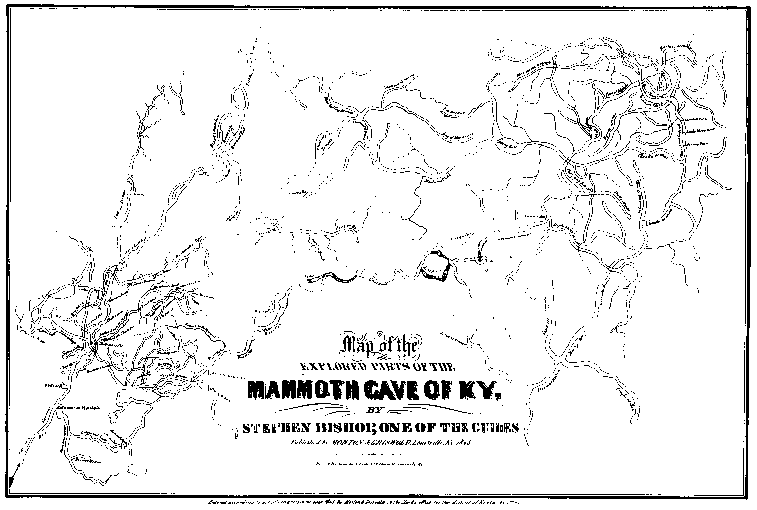
\includegraphics{MapofMammothCave.png}}

\end{frame}
\bframe{History, 1972-1981}
\begin{itemize}
\item Will Crowther
\item Explorer, Mammoth Cave
\item {\em Dungeons and Dragons} player
\item About 1972, wrote ADVENT for his children
\end{itemize}

\vspace{1cm}

{\bf At End of Road}

You are standing at the end of a road before a small brick building.
Around you is a forest.  A small stream flows out of the building
and down a gulley.

\end{frame}
\bframe{Crowther was a caver}

You are in a splendid chamber thirty feet high. The walls are frozen
rivers of orange stone. An awkward canyon and a good passage exit from
east and west sides of the chamber.

\end{frame}
\bframe{Parser Prehistory}

\begin{itemize}
\item Hunt the Wumpus
\item SHRDLU
\end{itemize}

\end{frame}
\bframe{History, 1972-1981}
\begin{itemize}
\item About 1975, Don Woods gets ahold of Crowther's ADVENT
\item Adds puzzles, pirates, vending machines {\em etc.}
\item ADVENT circulates on the ARPANET
\item {\em The Soul of a New Machine}, Tracy Kidder:  ADVENT
epitomizes the geek culture 
\item Scott Adams, many titles, simple games
\item John Laird's 'Haunt'
\item MUDs
\end{itemize}

\end{frame}

\bframe{Scott Adams}
\begin{multicols}{2}
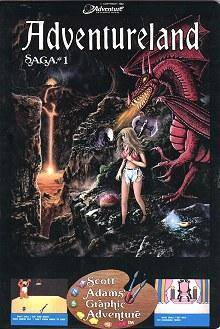
\includegraphics[width=0.5\textwidth]{Adventureland_Cover.png}
\columnbreak

Adventureland

1978

\vspace{2cm}

I'm in a dismal swamp.\\~\\

Obvious exits: North, South, East, West, Up.\\~\\

I can also see: cypress tree --- evil smelling mud --- swamp gas ---
floating patch of oily slime --- chiggers

\end{multicols}
\end{frame}

\bframe{1972-1981}

Game assemblers 

\begin{Verbatim}
JUMPHOLE:
 SKIP UNLESS R(CHAIR)R EQ HOLEROOM
 SKIP UNLESS H CHAIR PLAYER
 PRINTRET HOLEHIGH
 MOVE PLAYER WITH TO UPROOM
 PRINTRET CHAIRJUMP
\end{Verbatim}

\end{frame}
\bframe{1982-1986}

\begin{itemize}
\item MIT students built Zork
\item 1979, Started Infocom
\item Huge commercial success by 1985
\item Ran on over 20 different personal computer types
\item Business software never successful
\item Dozens of successful titles
\end{itemize}

\end{frame}
\bframe{Infocom}
\begin{multicols}{2}


\includegraphics[width=0.5\textwidth]{ZorkI.jpg}
\columnbreak

  \bi
  \item Enchanter, Sorcerer, Spellbreaker
  \item Deadline
  \item Suspended
  \item Infidel
  \item Planetfall
  \item Wishbringer
  \item Leather Goddesses of Phobos
  \item Trinity
  \ei
\end{multicols}

\end{frame}
\bframe{Sierra Online}

\resizebox{2.5in}{!}{
\includegraphics{LeisureSuitLarry.jpg}}

\end{frame}
\bframe{1982-1986}
The Golden Age
\begin{itemize}
\item {\it Amazon}, Michael Crichton
\item {\it The Hitchhiker's Guide to the Galaxy}, Douglas Adams
\item {\it Mindwheel}, Robert Pinsky (US Poet Laureate)
\item {\it I Have No Mouth and I Must Scream}, Harlan Ellison
\item {\it Gateway}, Frederik Pohl
\end{itemize}

\end{frame}
\bframe{1985-1991}
\begin{itemize}
\item Computer graphics improve
\item Market dries up
\item Infocom collapses, bought by Activision
\item Community grows  {\tt ftp.gmd.de}
\end{itemize}

\end{frame}
\bframe{1992-1999}
\begin{itemize}
\item TADS and Inform
\item Activision releases {\bf Lost Treasures of Infocom}
\item Newsgroups and the web
\item Annual contests:
\begin{itemize} 
\item GAGS (AGT) contest
\item XYZZY awards
\item SpeedIF (write a game in two hours)
\end{itemize}
\end{itemize}

\end{frame}
\end{document}
